\documentclass[uplatex,dvipdfmx,a4j,11  pt]{jsarticle}

\usepackage[utf8]{inputenc}
\usepackage{amsmath,amsfonts}
\usepackage{bm}
\usepackage{amssymb}
\usepackage{otf}
\usepackage{pxrubrica}
\usepackage{ascmac}
\usepackage{wrapfig}
\usepackage{here}
\usepackage[hang,small,bf]{caption}
\usepackage[subrefformat=parens]{subcaption}
\captionsetup{compatibility=false}

\usepackage{graphicx}
\usepackage{comment}
\usepackage{color}
\usepackage{url}
\usepackage{siunitx}
\usepackage[version=4]{mhchem}
\usepackage{paralist}
\usepackage{longtable}
\usepackage{multirow}
\usepackage[dvipdfmx]{hyperref}
\usepackage{pxjahyper}

\usepackage{fancyhdr}
\usepackage{lastpage}
\fancypagestyle{mypagestyle}{%
\lhead{}%ヘッダ左を空に
\rhead{}%ヘッダ右を空に
\cfoot{\thepage/\pageref*{LastPage}}%フッタ中央に"今のページ数/総ページ数"を設定
\renewcommand{\headrulewidth}{0.0pt}%ヘッダの線を消す
}
\pagestyle{mypagestyle}

% コマンド定義
\newcommand{\divergence}{\mathrm{div}\,}  %ダイバージェンス
\newcommand{\grad}{\mathrm{grad}\,}  %グラディエント
\newcommand{\rot}{\mathrm{rot}\,}  %ローテーション
\newcommand{\diff}{\mathrm{d}} % 微分
\newcommand{\e}{\mathbf{e}} % 単位ベクトル

\hypersetup{
  hidelinks,
  bookmarksnumbered=true
}

\title{減衰モーメント係数について}
\date{}
\author{佐藤 空馬 (14期代空力班長)}

\begin{document}
\maketitle
\thispagestyle{mypagestyle}%タイトルページ等ではpagestyleが変更されるので改めて設定する
\setcounter{section}{-1}
\section{はじめに}
この資料は, 弊団体で用いている\emph{ピッチ・ヨー減衰モーメント係数} (pitch/yaw damping moment coefficient) $C_{mq}$ 及び\emph{ロール減衰モーメント係数} (roll damping coefficient) $C_{mp}$ の計算式 : 
\begin{gather}
  C_{mq} = - 4 \sum_i \left(\frac{C_{n\alpha i}}{2}\right)\left(\frac{C_{pi} - C_{g}}{L}\right)^2,\label{pitch_damping_coef}\\
  C_{mp} = - 8 \times \cfrac{\left(\mathrm{span} + d/2\right)^4}{\pi L^2 \cfrac{\pi d^2}{4}} \label{roll_damping_coef}
\end{gather}
の導出を明らかにしたものです.

資料作成に当たっては, 「飛しょう体の空気力学」(玉木 著) \cite{aerodynamics}の第9章 安定微係数とBarrowman法の元論文\cite{barrowman}を参照しています.
「飛しょう体の空気力学」は東北大学附属図書館本館にも納められているので, 詳しく知りたい方はそちらも参照してください.

\section{減衰モーメント係数とは何か}
空気中を飛翔するロケットは機体とは垂直方向に\emph{法線力} (normal force) \footnote{\emph{揚力} (lift force) は機体進行方向に垂直な力. 低迎角では概ね一致するが厳密には違うので注意.}を受けます.
機体各部からの法線力の合力を受ける力点のことを\emph{圧力中心} (center of pressure, CP) といいます.
圧力中心は一般に機体重心 (center of gravity, CG) よりも後方にあり, 飛翔するロケットは重心を回転中心にこの法線力によってモーメントを受けるのです.

ところでこのモーメントは, 法線力 (厳密には揚力) は\emph{迎角} (機体進行方向と機軸方向がなす角) が増大すればするほど, 迎角を減少させる方向に力ははたらきます (\emph{風見効果}).
正確には, モーメントの減衰は角速度に比例するため (後述), 法線力はいわゆるマス-ダンパ系におけるダンパと同じはたらきをし, 法線力のモーメントによって迎角は振動減衰します.
この減衰振動の係数を\emph{減衰モーメント係数} (damping moment coefficient)といいます.

なお, ほぼ真上に打ち上げた際は機体が頂点前後で大きく回転するため大きく減衰振動しますが, そうでない場合はあまり振動現象はみられません.
そのため, 飛行シミュレーションソフト : Open Rocket の技術書\cite{openrocket}を見ると, 頂点付近でのみ効いてくるのであまりちゃんと考えなくてもいいよと書かれていたりします
\footnote{陸打ちでは往々にしてほぼ鉛直 ($\simeq 89\,\mathrm{[deg]}$) で打ち上げるので, 個人的には, 減衰モーメント係数が微小かつ無風のときは頂点--落下時に割とクリティカルに効いてくると思います.}:
\begin{quote}
  Since the pitch damping moment is notable only at apogee, and therefore does
not contribute to the overall flight characteristics, only a rough estimate of its
magnitude is required.
\end{quote}

\enskip

さて, より具体的にはピッチ・ヨー角における減衰モーメント係数 (ピッチ角とヨー角は対称性から一致する) と, 機体が回転することでフィンに迎角が与えられて生じるロール方向の減衰モーメント係数が考えられます.

定義から, 一般の減衰モーメント係数$C_{m\dot{\theta}}$は
\begin{equation}
  C_{m\dot{\theta}} = \frac{4}{\rho v^2 S L}\frac{v}{L}\frac{\partial M}{\partial\dot{\theta}} \label{fte_def}
\end{equation}
であって, ピッチ・ヨー減衰モーメント係数$C_{mq}$, ロール減衰モーメント係数$C{mp}$は (再掲):
\begin{gather*}
  C_{mq} = - 4 \sum_i \left(\frac{C_{n\alpha i}}{2}\right)\left(\frac{C_{pi} - C_{g}}{L}\right)^2,\tag{\ref{pitch_damping_coef}}\\
  C_{mp} = - 8 \times \cfrac{\left(\mathrm{span} + d/2\right)^4}{\pi L^2 \cfrac{\pi d^2}{4}} \tag{\ref{roll_damping_coef}}
\end{gather*}
と, 団体内資料にありました. ですが, その詳細は謎でした. 

そこで次の章からは, この式の導出を行っていきます.

\section{安定微係数}
\subsection{座標系と記号の導入}
ここでは, 機体座標系を用います.

つまり, 機軸方向前向きを$X$正の向き, 原点を機体重心とし, 水平方向に$Y$軸を, $X, Y$軸と垂直で右手系をなすように$Z$軸を採ります.
また, 参考文献\cite{aerodynamics}に倣い, $X, Y, Z$軸からの力をそれぞれ$X, Y, Z$で表記します

さらに, 各軸周りの回転角を$\phi, \theta, \psi$とし\footnote{厳密には回転の順序によって結果が異なりますが, ここではある空間固定した座標系からの微小変化とします. この場合は回転の順序など複雑なことを考える必要がありません.},
角速度を$p, q, r$とします.
つまり, $\phi$がロール角, $\theta$がピッチ角, $\psi$がヨー角に対応します.

また, 各軸周りのモーメントはそれぞれ$L$, $M$, $N$とします.

静止系からの機体重心の速度はそれぞれ$u, v, w$, その大きさを$V_0$とします.
当たり前ですが, 機体の運動$u, v, w$と機体の姿勢$\phi, \theta, \psi$に直接の関係はありません.

\subsection{安定微係数}
ここでは, 空気力とモーメントは速度$u, v, w$と角速度$p, q, r$の関数と仮定します.

始めにロール方向のモーメント$L$のTaylor展開を考えます.
これは, 先の仮定に基づけば,
\begin{equation}
  L \equiv L(u, v, w, p, q, r)
\end{equation}
と表され, これを1次の項まででTaylor展開すると,
\begin{equation}
  L = L_0 + \frac{\partial L}{\partial u}\delta u + \frac{\partial L}{\partial v}\delta v + \frac{\partial L}{\partial w}\delta w + \frac{\partial L}{\partial p}\delta p + \frac{\partial L}{\partial q}\delta q + \frac{\partial L}{\partial r}\delta r
\end{equation}
と展開できます. 
ここで$u, v, w, p, q, r$それぞれで偏微分した値を微係数といいます.
また, 力$X, Y, Z$, モーメント$L, M, N$の微係数36個の内, 
特に$u, v, w$に関するものをresistance stability derivatives (抵抗安定微係数?), 
$p, q, r$に関するものをrotary stability derivatives (回転安定微係数?)といいます
\footnote{他にも加速度, 角加速度に関するものをacceleration stability derivatives (加速度安定微係数?) と呼びます.}.

\enskip

議論を簡単にするために, 各パラメータを無次元化してきます.
まず初めに, 基準長を$\lambda$, 基準面積を$S_{R}$, 主流動圧を$q_0$とします.

力を無次元化すると,
\begin{equation}
  C_X = \frac{X}{q_0S_R}, \quad
  C_Y = \frac{Y}{q_0S_R},  \quad
  C_Z = \frac{Z}{q_0S_R}, \label{force_nondimentional}
\end{equation}
モーメントを無次元化すると,
\begin{equation}
  C_m = \frac{M}{q_0S_R\lambda}, \quad
  C_n = \frac{n}{q_0S_R\lambda}, \quad
  C_l = \frac{l}{q_0S_R\lambda}
\end{equation}
となります
\footnote{それぞれ軸力 / 法線力係数, モーメント係数と言います.}.

さらに速度を無次元化して,
\begin{equation}
  \frac{u}{V_0}, \quad \beta=\frac{v}{V_0} \text{(横滑り角)}, \quad \alpha = \frac{w}{V_0} \text{(迎角)},\label{velocity_nondimentional}
\end{equation}
角速度を無次元化して,
\begin{equation}
  \frac{p\lambda}{2V_0}, \quad
  \frac{q\lambda}{2V_0}, \quad
  \frac{r\lambda}{2V_0}\footnotemark
\end{equation}
\footnotetext{角速度を$V_0/(\lambda/2)$で除しているのは$\lambda/2$が代表的な重心からの長さであり, その点における角速度が$V_0/(\lambda/2)$であるためだと思います. なお\cite{aerodynamics}では第2式が$g\lambda/2V_0$となっていますが, 恐らく誤記です.}
となります.

\emph{安定微係数}は通常上のような無次元量の微係数に対して考えられます.

ここでは, 本題であるピッチ角とヨー角に関する減衰モーメント係数に関連するものをピックアップして考えます.

それぞれピッチ角$q$, ロール角$p$に関連してモーメント$M$, $L$の安定微係数を考えればよく,
\begin{gather}
  C_{mq} = \frac{\partial C_m}{\partial (q\lambda/2V_0)},
  C_{lr} = \frac{\partial C_l}{\partial (r\lambda/2V_0)}\label{damping_moment_coef}
\end{gather}
がピッチ減衰モーメント係数 (\cite{aerodynamics}では damping in pitch), ロール減衰モーメント係数 (\cite{aerodynamics}ではdamping in roll)となります.
なお, $C_m = M/q_0S_R\lambda = 2M/\rho v^2 S_R \lambda$ \, ($\because q_0 \equiv \rho v^2 /2$)を用いれば, 確かに弊団体内資料の式(\ref{fte_def})と一致します
(式(\ref{fte_def})では代表長さが$L$なことに注意).

\section{ロール減衰モーメント係数の導出}

\subsection{細長体理論 (slender-body theory)}
ここでは細長い物体に適用できる\ruby{細長体}{さい|ちょう|たい}理論 (slender-body theory) と見かけの質量 (apparent mass) という考え方を用いてロール方向の安定微係数を解析的に考えます.

ここで$X = X_c$で切り取った機体断面平面を考えます.
この平面上で$Y, Z$軸に平行な速度成分を$v_1, v_2$とし, $X$軸周りの角速度を$p$とします.

$v_1, v_2, p$の単位量あたりのポテンシャルを$\phi_1, \phi_2, \phi_3$と書くと, 全体のポテンシャルは次で表されます.
\begin{equation}
  \phi = v_1 \phi_1 + v_2 \phi_2 + p \phi_3\footnotemark. \label{potential_def}
\end{equation}
\footnotetext{ここで機体断面が広がる方向について$\log$で比例する項は無視しています. 果たして一般にこのように書いて問題ないのか分からないので, 分かる方教えてください.}


$X = X_c$における$X$軸方向単位長さあたりの運動エネルギー$T$を考えます.
単位体積あたりのエネルギーが,
\begin{align}
  \frac{1}{2}\rho v^2 = \frac{1}{2}\rho \left(\nabla\mathbf{v}\right)^2 = \frac{1}{2}\phi\nabla\phi
\end{align}
なので(ポテンシャル流より$\nabla^2\phi=0$), これの単位長さあたりを考えると,
\begin{equation}
  T = - \frac{1}{2} \rho \oint_C \frac{\partial \phi}{\partial \mathbf{n}} \diff s
\end{equation}
となります.
ここで, $C$は$X=X_C$における機体断面の周囲, $s$は$C$の線素, $\mathbf{n}$はこの機体断面に垂直な法線ベクトルです
\footnote{ここでは面からの湧き出しということで方向微分に置き換えています. 法線ベクトルの採り方によって正負が決まるのですが, 何故マイナスが付くのか自信をもって説明できないので分かる方教えてください.}.

式(\ref{potential_def})より, $T$は次のように表すことができます :
\begin{align}
  -\frac{T}{\rho S_R / 2} = &\frac{v_1^2}{S_R}\oint_C\phi_1\frac{\partial \phi_1}{\partial\mathbf{n}}\diff s
  + \frac{v_1 v_2}{S_R}\oint_C\phi_1\frac{\partial \phi_2}{\partial\mathbf{n}}\diff s
  + \frac{v_1 (\lambda p)}{\lambda S_R}\oint_C\phi_1\frac{\partial \phi_3}{\partial\mathbf{n}}\diff \\
  + &\frac{v_1 v_2}{S_R}\oint_C\phi_1\frac{\partial \phi_1}{\partial\mathbf{n}}\diff s
  + \frac{v_2^2}{S_R}\oint_C\phi_1\frac{\partial \phi_2}{\partial\mathbf{n}}\diff s
  + \frac{v_2 (\lambda p)}{\lambda S_R}\oint_C\phi_1\frac{\partial \phi_3}{\partial\mathbf{n}}\diff \\
  + &\frac{v_1 v_3}{S_R}\oint_C\phi_1\frac{\partial \phi_1}{\partial\mathbf{n}}\diff s
  + \frac{v_2 (\lambda p)}{\lambda S_R}\oint_C\phi_1\frac{\partial \phi_2}{\partial\mathbf{n}}\diff s
  + \frac{(\lambda p)^2}{\lambda^2 S_R}\oint_C\phi_1\frac{\partial \phi_3}{\partial\mathbf{n}}\diff .
\end{align}
(次元を合わせるために$\lambda$を導入している)

ここで, 上式の積分を慣性係数 (inertia coefficient) といい, $A_{ij}$で表します:
\begin{equation}
  \begin{pmatrix}
    A_{11} & A_{12} & A_{13}\\
    A_{21} & A_{22} & A_{23}\\
    A_{31} & A_{32} & A_{33}
  \end{pmatrix}
  = 
  \begin{pmatrix}
    \frac{1}{S_R}\oint_C\phi_1\frac{\partial \phi_1}{\partial\mathbf{n}}\diff s &
    \frac{1}{S_R}\oint_C\phi_1\frac{\partial \phi_2}{\partial\mathbf{n}}\diff s &
    \frac{1}{\lambda S_R}\oint_C\phi_1\frac{\partial \phi_3}{\partial\mathbf{n}}\diff \\
    \frac{1}{S_R}\oint_C\phi_1\frac{\partial \phi_1}{\partial\mathbf{n}}\diff s &
    \frac{1}{S_R}\oint_C\phi_1\frac{\partial \phi_2}{\partial\mathbf{n}}\diff s &
    \frac{1}{\lambda S_R}\oint_C\phi_1\frac{\partial \phi_3}{\partial\mathbf{n}}\diff \\
    \frac{1}{S_R}\oint_C\phi_1\frac{\partial \phi_1}{\partial\mathbf{n}}\diff s &
    \frac{1}{\lambda S_R}\oint_C\phi_1\frac{\partial \phi_2}{\partial\mathbf{n}}\diff s &
    \frac{1}{\lambda^2 S_R}\oint_C\phi_1\frac{\partial \phi_3}{\partial\mathbf{n}}\diff .
  \end{pmatrix}.
\end{equation}

これはGreenの第二定理 : $\displaystyle \int_S (\psi \phi_\mathbf{n} - \phi \psi_\mathbf{n})\diff S = \int_V (\psi\nabla^2\phi - \phi\nabla^2\psi)\diff V$から, $\nabla^2\phi = \nabla^2\psi=0$とし, $V$の厚さを$0$に近づけることで\footnote{正当化されるのか微妙.},
\begin{equation}
  \oint_C \phi_i \frac{\partial\phi_j}{\partial \mathbf{n}} =
  \oint_C \phi_j \frac{\partial\phi_i}{\partial \mathbf{n}},
\end{equation}
つまり, 
\begin{equation}
  A_{ij} = A_{ji}
\end{equation}
が成り立つことが分かります (つまり対称テンソル).

ちなみに, 系が軸対称形の場合は軸対称な点同士で積分が相殺されるので, 非対角成分は$0$になると思われます.

また特に, 底面$X = X_b$における値を$\bar{A}_{ij}$で表記します.

\enskip

この慣性係数$A_{ij}$と, これらを機軸方向 ($X$軸方向) で$X = X_b$ (底面) から$X = X_n$ (ノーズ) まで (正規化して) 積分した値:
\begin{equation}
  \left\{ 
  \begin{alignedat}{2}  
    \,&B_{ij} = \int_{(X/\lambda)_b}^{(X/\lambda)_n} A_{ij}\,\diff\left(\frac{X}{\lambda}\right),\\
    \,&C_{ij} = \int_{(X/\lambda)_b}^{(X/\lambda)_n} A_{ij}\left(\frac{X}{\lambda}\right)\,\diff\left(\frac{X}{\lambda}\right),\\
    \,&D_{ij} = \int_{(X/\lambda)_b}^{(X/\lambda)_n} A_{ij}\left(\frac{X}{\lambda}\right)^2\,\diff\left(\frac{X}{\lambda}\right)
  \end{alignedat} 
  \right.
\end{equation}
を用いることで, ロール減衰モーメント係数$C_{lr}$を表すことができます.

計算は煩雑なので途中式は飛ばしますが, 結論だけ述べると,
\begin{equation}
  C_{lr} = -4 \bar{A}_{33} + 4 \alpha B_{13} - 4 \beta b_{23} - 8 \left(\frac{\lambda q}{2 V_0}\right) C_{13} - 8 \left(\frac{\lambda r}{2V_0}\right) C_{23}
\end{equation}
となります.

\subsection{見かけの質量 (apparent mass)}

ここでは見かけの質量 (apparent mass)\footnote{もしくは有効質量 (effective mass).} $m_{ij}$ という考え方を使います:
\begin{equation}
  m_{ij} \equiv -\rho\oint_C \phi_i \frac{\partial \phi_j}{\partial\mathbf{n}}\diff S
\end{equation}

これを使うと以下のように表せます.
\begin{equation}
  \left\{ 
  \begin{alignedat}{2}
    \,&A_{11} = \frac{m_{11}}{\rho S_R}\\
    \,&A_{12} = \frac{m_{12}}{\rho S_R}\\
    \,&A_{13} = \frac{m_{13}}{\rho \lambda S_R}\\
    \,&A_{22} = \frac{m_{22}}{\rho S_R}\\
    \,&A_{23} = \frac{m_{23}}{\rho \lambda S_R}\\
    \,&A_{33} = \frac{m_{33}}{\rho \lambda^2 S_R}
  \end{alignedat} 
  \right.
\end{equation}

ここで注目すべきは, 位置$X$に依存するはずの$A_{ij}$が依存せずに一定になるという点です.

さらに, 十字翼・円筒体 (cruciform wing, circular body) における見かけの質量 は以下のようになります.
\begin{equation}
  \left\{ 
  \begin{alignedat}{2}
    \,&m_{11} = \pi \rho s^2 \left(1 - \frac{a^2}{s^2} + \frac{a^4}{s^4}\right),\\
    \,&m_{12} = 0,\\
    \,&m_{13} = 0,\\
    \,&m_{22} = \pi \rho s^2 \left(1 - \frac{a^2}{s^2} + \frac{a^4}{s^4}\right),\\
    \,&m_{23} = 0,\\
    \,&m_{33} = \frac{2\rho s^4}{\pi}\quad  \text{if}\, a = 0,\\
    \,&m_{33} : \text{numerical}\quad \text{if}\, a \ne 0
  \end{alignedat} 
  \right.
\end{equation}
ここで$a$は機体半径, $s$は機軸から翼端までの距離 (つまり$a + \text{フィンスパン長(高さ)}$).

以上を用いれば, 十字翼・円筒体におけるロール減衰モーメント係数を求められます :
\begin{align}
  C_{lr} &= -4 \bar{A}_{33} + 4 \alpha B_{13} - 4 \beta b_{23} - 8 \left(\frac{\lambda q}{2 V_0}\right) C_{13} - 8 \left(\frac{\lambda r}{2V_0}\right) C_{23}\nonumber\\
  &= -\bar{A}_{33} = -4\frac{m_{33}}{\rho\lambda^2 S_R}
  % &= - = - 8 \frac{s^4}{\pi\lambda^2S_R}\nonumber\\
  % &= -8 \frac{(\text{span} + d/2)^4}{\pi L^2 \pi d^2/4}
\end{align}

ここで, $a = 0$における値については容易に計算することができ,
\begin{equation}
  (C_{lr})_{a = 0} =  -4\frac{(m_{33})_{a = 0}}{\rho\lambda^2 S_R}= -8 \frac{(\text{span} + d/2)^4}{\pi L^2 \pi d^2/4}
\end{equation}
を得ます.
ここで, $a \to d / 2$, $\lambda \to L$, $S_R \to \pi d^2/4$としています.

これで目的の式を得ました.
これから分かるのは, 弊団体で用いている式は機体半径$a = 0$における式だったのです.

\enskip

しかしこの式は別に$a \ne 0$においても十分に成り立ちます.

ここで, $a = 0$におけるロール減衰モーメント係数からの比$C_{lr}/(C_{lr})_{a = 0} = m_{33}/(m_{33})_{a = 0}$は, 機体半径をスパン長と機体半径の和で除した$a/s$の関数とみることができます.
十字翼における$C_{lr}/(C_{lr})_{a = 0}$の値については例えばAdaumとDuganによる数値計算による値が知られており\cite{roll_damping_moment_est}
\footnote{AdaumとDugan \cite{roll_damping_moment_est}ではフィンのアスペクト比で議論しています. ここでは簡便のためにNielsen \cite{nielsen1988missile}を参考に$a/s$で考えます.},
Nielsen \cite{nielsen1988missile} から図を引用すると, 図\ref{damping_vs_radius}のようになります.
\begin{figure}[htbp]
  \centering
  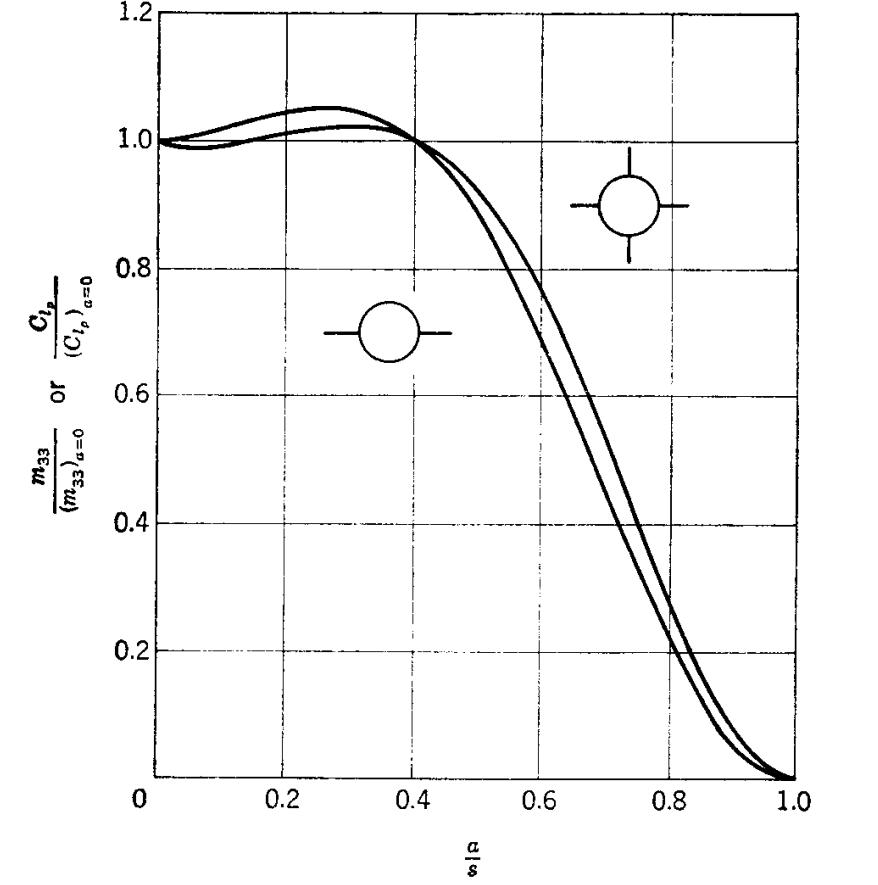
\includegraphics[width=80mm]{damping_moment/img/damping_coeff.png}
  \caption{機体半径がロール減衰モーメント係数に及ぼす影響 (\cite{nielsen1988missile}より図引用).}
  \label{damping_vs_radius}
\end{figure}

したがって, フィンスパン長が機体半径の2倍よりも長い場合はロール減衰モーメント係数は概ね$a = 0$のときの値と一致すると言えます.

参考までに, KSE2024陸打ちの``たんぽぽ''の$a/s$は$0.45$, NSE2024陸打ちの``火垂''の$a/s$は$0.43$, 同海打ちの``みかん''は$0.55$でした.
そのため, これらのケースでは$C_{lr}/(C_{lr})_{a = 0} = 0.8 \sim 1.0$程度であり, かなり良い精度で一致していることが分かります.


\section{ピッチ・ヨー減衰モーメント係数の導出}
ピッチ・ヨー減衰モーメント係数の定義式は (再掲),
\begin{equation}
  C_{mq} \equiv \frac{\partial C_m}{\partial (qL/2V_0)}\tag{\ref{damping_moment_coef}}
\end{equation}
でした (ここで代表長さを$\lambda$から$L$に直しています).
ここでは, ピッチ角に注目して減衰モーメント係数を考えていきます.

\enskip

以下, 各コンポーネント (ノーズ, ボディ, フィン, テール, ヴォルテックス・ジェネレータ (VG), etc.) を添え字$i$で区別します.

ピッチ方向のモーメント$M$は, 各部にかかる空力的な力$F_i$と, 重心から力点 (圧力中心) までの距離 $\Delta x_i$ の総和として, 次で表されます:
\begin{equation}
  M = \sum_i F_i \Delta x_i.
\end{equation}
ここで, $\Delta x_i$は, 機体先端からの重心位置$C_g$と圧力中心位置$C_{pi}$を用いて,
\begin{equation}
  \Delta x_i \equiv C_{pi} - C_g 
\end{equation}
です.

また, $F_i$は, 迎角$\alpha$における法線力係数$C_{n\alpha}$
\footnote{力を無次元化した式\eqref{force_nondimentional}の第3式と同じ.}
が$C_{n i} \equiv C_{n\alpha i} \alpha$であることから, 
\begin{equation}
  F_i = - C_{n\alpha i} \alpha q_0 S_R
\end{equation}
となります.
ここで$q_0$は動圧, $S_R$は代表断面積で, 迎角$\alpha$の増加する向きと法線力の向きは反対なのでマイナス符号が付いています.

さて, 迎角$\alpha$は低迎角$\alpha \ll 1$において (再掲), 
\begin{equation}
  \alpha \simeq \frac{w}{V_0} \tag{\ref{velocity_nondimentional}}.
\end{equation}
近似的に速度$w$は
\begin{equation}
  w \simeq q \Delta x_i
\end{equation}
なので, 以上の式を纏めると, 次のようになります:
\begin{equation}
  F_i = - C_{n\alpha i} q_0 S_R\frac{q\Delta x_i}{V_0}.
\end{equation}

したがって, ピッチ方向のモーメントは,
\begin{equation}
  M = -\sum_i C_{n\alpha i} (\Delta x)^2 S_R q_0 \frac{q}{V_0}.
\end{equation}
つまり, モーメント係数は,
\begin{equation}
  C_{m} \equiv \frac{M}{q_0 S_R L} = - \sum_i C_{n\alpha i} \frac{(\Delta x)^2}{L} \frac{q}{V_0} = - 2\sum_i C_{n\alpha i} \left(\frac{C_{pi} - C_g}{L}\right)^2 \frac{q L}{2V_0}.
\end{equation}

よって, ピッチ減衰モーメント係数$C_{mq}$は,
\begin{equation}
  C_{mq} \equiv \frac{\partial C_m}{\partial (qL/2V_0)} = - 2\sum_i C_{n\alpha i} \left(\frac{C_{pi} - C_g}{L}\right)^2
\end{equation}
となり, 確かにピッチ・ヨー方向の減衰モーメント係数を得られました
\footnote{余談として, 以上の導出は\cite{barrowman}に基づいているのですが, 何故か最後の結論の式 (3-115) だけ抜けています. ``Thus, using equation 3-113 in 3-114.''まで書いて何故...}.


\bibliography{damping_moment/bib/ref}
\bibliographystyle{junsrt}

\end{document}